\documentclass{standalone}
\usepackage{tikz}
\begin{document}
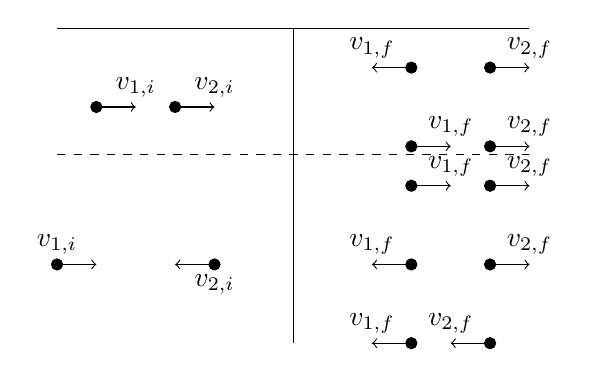
\begin{tikzpicture}[scale=2]
    \draw[-](-1.5,1)--(1.5,1);
    \draw[-](0,1)--(0,-1);

    \draw[->](-1.25,0.5)--(-1,0.5)node[above]{$v_{1,i}$};
    \draw[->](-0.75,0.5)--(-0.5,0.5)node[above]{$v_{2,i}$};

    \draw[->](0.75,0.25)--(1,0.25)node[above]{$v_{1,f}$};
    \draw[->](1.25,0.25)--(1.5,0.25)node[above]{$v_{2,f}$};
    \draw[->](0.75,0.75)--(0.5,0.75)node[above]{$v_{1,f}$};
    \draw[->](1.25,0.75)--(1.5,0.75)node[above]{$v_{2,f}$};

    \draw[dashed](-1.5,0.20)--(1.5,0.20);

    \draw[<-](-1.25,-0.5)--(-1.5,-0.5)node[above]{$v_{1,i}$};
    \draw[<-](-0.75,-0.5)--(-0.5,-0.5)node[below]{$v_{2,i}$};

    \draw[->](0.75,0)--(1,0)node[above]{$v_{1,f}$};
    \draw[->](1.25,0)--(1.5,0)node[above]{$v_{2,f}$};
    \draw[->](0.75,-0.5)--(0.5,-0.5)node[above]{$v_{1,f}$};
    \draw[->](1.25,-0.5)--(1.5,-0.5)node[above]{$v_{2,f}$};
    \draw[->](0.75,-1)--(0.5,-1)node[above]{$v_{1,f}$};
    \draw[->](1.25,-1)--(1,-1)node[above]{$v_{2,f}$};

    \filldraw[black](-1.25,0.5)circle(1pt);
    \filldraw[black](-1.5,-0.5)circle(1pt);
    \filldraw[black](-0.75,0.5)circle(1pt);
    \filldraw[black](-0.5,-0.5)circle(1pt);
    \filldraw[black](0.75,0.25)circle(1pt);
    \filldraw[black](1.25,0.25)circle(1pt);
    \filldraw[black](0.75,0.75)circle(1pt);
    \filldraw[black](1.25,0.75)circle(1pt);
    \filldraw[black](0.75,0)circle(1pt);
    \filldraw[black](1.25,0)circle(1pt);
    \filldraw[black](0.75,-0.5)circle(1pt);
    \filldraw[black](1.25,-0.5)circle(1pt);
    \filldraw[black](0.75,-1)circle(1pt);
    \filldraw[black](1.25,-1)circle(1pt);
\end{tikzpicture}
\end{document}